\documentclass[12pt, fullpage,letterpaper]{article}

\usepackage[margin=1in]{geometry}

\usepackage{gensymb}
\usepackage{url}
\usepackage{amsfonts}
\usepackage{algorithmic}
\usepackage{graphicx}


\newcommand{\Z}{\mathbb{Z}}

\newcommand{\bw}{{\bf w}}
\newcommand{\bx}{{\bf x}}

\newcommand{\semester}{Fall 2016}
\newcommand{\assignmentId}{2}
\newcommand{\releaseDate}{Sep 13, 2016}
\newcommand{\dueDate}{Sep 27, 2016}

\title{CS 5350/6350: Machine Learining \semester}
\author{Homework \assignmentId}
\date{Handed out: \releaseDate\\
  Due date: \dueDate}

\begin{document}
\maketitle

\section{Warm up: Feature expansion}
We note that the function is not linearly separable in 2 dimensions. Therefore, we move to a representation in 3 dimensions such that, we can linearly separate the data.\\
Now, let us consider the third dimension as $z=4x_1^4 + 16x_2^4$. Now every point in this new dimension would be represented by $(x_1,x_2,4x_1^4 + 16x_2^4)$. The transformation function $\phi(x_1, x_2)=(x_1,x_2,4x_1^4 + 16x_2^4)$\\
To prove that in the new space, the positive and negative examples are linearly separable, let us try to find a hyperplane such that  $\bw^T\phi(x_1, x_2) \geq b$ if, and only if,
$f_r(x_1, x_2) = +1$.\\
If we can somehow, set the weights for $(x_1,x_2,4x_1^4 + 16x_2^4)$ such that $4x_1^4 + 16x_2^4 \leq r$, we would be able to prove that the positive and negative examples are linearly separable as we are setting the boundary in 3 dimensions.\\
For this, let us consider the "-r" as the bias(b) and the weights(w) to be [0  0 -1] for $(x_1,x_2,4x_1^4 + 16x_2^4)$. Therefore, $\bw^T\phi(x_1, x_2) \geq b$ would be the same as $4x_1^4 + 16x_2^4 \leq r$. Therefore, this matches with the equation in the question. 
Thus we can say that $\bw^T\phi(x_1, x_2) \geq b$  equivalent to $4x_1^4 + 16x_2^4 \leq r$ if, and only if,
$f_r(x_1, x_2) = +1$. Also $\bw^T\phi(x_1, x_2) < b$ equivalent to $4x_1^4 + 16x_2^4 > r$ if, and only if,
$f_r(x_1, x_2) = -1$.  Hence we have been able to represent the same problem in 3 dimensions which is now linearly separable.

\section{Mistake Bound Model of Learning}
1.\\
Each function $f_r$ in C is defined by $r$ (with
$1 \leq r \leq 80$). Therefore, r can take values from 1 to 80, and thus 80 functions can be defined by the radius r which is the size of the concept class. Therefore, the size of the concept class, $|C|=80$.\\\\
2.\\
For the correct prediction(+1) of a  positive example, $ x_1^2 + x_2^2 \leq r^2$  i.e., $ x_1^2 + x_2^2 - r^2 \leq 0$. Similarly for a negative example, the correct prediction(-1) is made when $ x_1^2 + x_2^2 - r^2 > 0$\\
Therefore, for the correct prediction for a particular example "t" is made, the product of the guess ($x_1^{t^2} + x_2^{t^2} - r^2$) and the actual label ($y^t$) is always $\leq 0$. Hence a mistake is made when the product of the guess and label is $>0$.\\
Mathematically, a mistake is made when ($(x_1^{t^2} + x_2^{t^2} - r^2)*y^t)>0$ for a particular example t.\\\\
3.\\
As mentioned, if there is an error, we only need to update r as $f_r$ is only dependent on r.\\
We also know that r is an integer(posted in discussion forum) with $1 \leq r \leq 80$.
\\For a positive example, an error is made when $ x_1^2 + x_2^2 > r^2$ i.e., $r^2<x_1^2 + x_2^2  $. Therefore r needs to be set correctly after every mistake. Therefore, for every positive example, if a mistake is made on an example t, r needs to be incremented with the following update:\\
$r_{t+1}=r_t+1$\\
Similarly for a negative example, an error is made when $ x_1^2 + x_2^2 <= r^2$ i.e., $r^2>=x_1^2 + x_2^2  $, r needs to be decremented using the following update:\\
$r_{t+1}=r_t-1$\\
We are increasing/decreasing r by 1 because r can only be an integer. \\
Therefore, if $y_t$ is the label, then in case of a mistake, we can make the update as $r_{t+1}=r_t+y_t$.
\\\\
4.\\
Pseudo-code for Mistake Bound Learning Algorithm mentioned above:\\
START\\
SET r to RANDOM(1,80) /* Set r to a random integer between 1 and 80*/\\
FOR each example t in training data\\
SET $err=((x_1^{t^2} + x_2^{t^2} - r^2)*y^t)$     /*  where $y^t$ is the actual label for the particular example*/\\
IF err$>0$ THEN\\
SET $r=r+y_t$\\
END IF\\
END FOR\\
RETURN r\\
STOP\\
We know that r can take integer values between 1 to 80. This means that the worst cases would be\\
- when we the actual r is 80 and we intitalize r to 1\\
- when the actual r is 1 and we initialize r to 80\\
Therefore the maximum number of mistakes is given by $|C|-1$ in this case. Therefore, it is 80-1=79\\\\
5.\\
a) The set of hypothesis  with all examples seen so far can be given with 2 integers.\\
Suppose, when a particular example t arrives, say the majority predicts +1 and it is a mistake. Now, with the halving algorithm, we would only keep those elements that agree with t, i.e., all functions that agree with $ x_1^2 + x_2^2 > r^2$. This gives,  $r<\sqrt{x_1^{t^2} + x_2^{t^2}}$. Let us call this r1. SImilarly, when a particular example t arrives, say the majority predicts -1 and it is a mistake. Now, with the halving algorithm, we would only keep those elements that agree with t, i.e., all functions that agree with $ x_1^2 + x_2^2 \leq r^2$. This gives,  $r\geq \sqrt{x_1^{t^2} + x_2^{t^2}}$. Let us call this r2. Now, we know that r can only go between 1 to 80 and we have values of r1 and r2 which specify the limits for the hypothesis consistent with the examples seen so far. Therefore, the 2 integers required to be stored are r1 and r2.\\\\
b) For an example $(x_1^t, x_2^t)$, we will first see what the majority of the functions in the concept class predict. Let us say they predict 'p'. If the actual label $y^t$ is not equal to p, then there is an error.\\\\
c) Halving algorithm for this concept space.\\
START
\\1. Initialize $C=C_o$ /* the set of all possible functions defined by $f_r$ where $1\leq r\leq80$*/\\
Initalize r1=1; r2=80\\
2. For each  example t that arrives:\\
a) Predict the label of x as +1 if the majority of the functions $f_r$ predict +1, otherwise predict -1. Call this prediction $p_t$.\\
b) If $p_t$ is not equal to $y_t$(actual label of the example), then\\
i) If $p_t$ is +1, SET $r2=\lceil \sqrt{x_1^{t^2} + x_2^{t^2}} \rceil$    /*keep only those $f_r$ with $r<\sqrt{x_1^{t^2} + x_2^{t^2}}$*/\\
ii) If $p_t$ is -1,  SET $r1=\lfloor \sqrt{x_1^{t^2} + x_2^{t^2}} \rfloor$    /*keep only those $f_r$ with $r>\sqrt{x_1^{t^2} + x_2^{t^2}}$*/\\
3. Continue until r1=r2 i.e., only one $f_r$ remains in C.\\
STOP
\\\\
Mistake bound for this algorithm:\\
Suppose the algorithm makes n mistakes and we have a final set of concepts with 1 element i.e., $C_n=1$ ..................1\\
We know that with every mistake at least half of the functions in in the concept class C is are dropped by updating either r1 or r2. Therefore,\\
$|C_n|<1/2 |C_{n-1}| \\
|C_n|<1/2 * 1/2 * |C_{n-2}| $\\
This finally gives,\\
$|C_n|<1/2^n * |C_o| = |C_n|<1/2^n * |C|$...............2\\
From 1 and 2,
$|C|>2^{n}$ which gives n$<log|C|$\\
Therefore, $log|C|$ is the maximum number of mistakes where $|C|$ is the size of the concept class.


\section{Perceptron Algorithm and It's Variants}
\setcounter{subsection}{2}
\subsection{Algorithms}
\emph{Please note that each unique combination of the hyper-parameters in the following questions have been run over 50 times and taken an average of due to the random initialization of weights. For the exhaustive data for each run, please refer to the following folder-"Outputs/OutputData".\\
These execution would take several minutes. Therefore, for the code submitted, I have reduced the number of iterations, and also the number of values considered for hyper-parameters have been reduced. To run the exhaustive cases, please find instructions in README.}\\\\
1. \\
The program reads the input and converts it into a matrix form.
It then checks if  if $y (\bw^T\bx + b) <= 0$ and makes the following updates only the condition is true.\\
$\bw_{new} \leftarrow \bw_{old} + r y \bx$\\
$b_{new} \leftarrow b_{old} + r y$.\\\\
On running the perceptron algorithm by initializing the weights and  the bias to 0, and keeping the \textbf{rate as 1}, we get the following:\\
Number of mistakes=4\\
Weight vector(\textbf{w}): 0  0  1  0  -1  2\\
Bias(b)=0\\\\
On decreasing the rate, it is noticed that the weight vector value changes in proportion to the rate value. However, the number of mistakes remain the same.\\
On taking the \textbf{rate as 0.25},\\
Number of mistakes=4\\
Weight vector(\textbf{w}): 0.0  \hspace{5pt} 0.0  \hspace{5pt}0.25 \hspace{5pt} 0.0 \hspace{5pt}-0.25 \hspace{5pt}	0.5\\
Bias(b)=0\\\\
2.\\
For this problem, I ran the program by training on the train data, and testing on both train and the test data.\\
The program was run for every combination or rate(r) and margin(u). I changed the rate to 0.01, 0.001 and from 0 to 1 in increments of 0.1, and changed margin from 0(normal perceptron) to 5 in increments of 0.5.\\
Also, since the random initialization of weights were giving different values, I ran each combination of rate and margin for 50 times. Therefore the accuracy and the number of mistakes' values that I have mentioned is the average accuracy and the average number of mistakes over the 50 runs along with its standard deviation, all other hypermarameters remaining the same.\\
The below data summarizes the run. I have attached the raw output for individual runs along with the code in "Outputs/OutputData(3.3.2)" for more details.\\
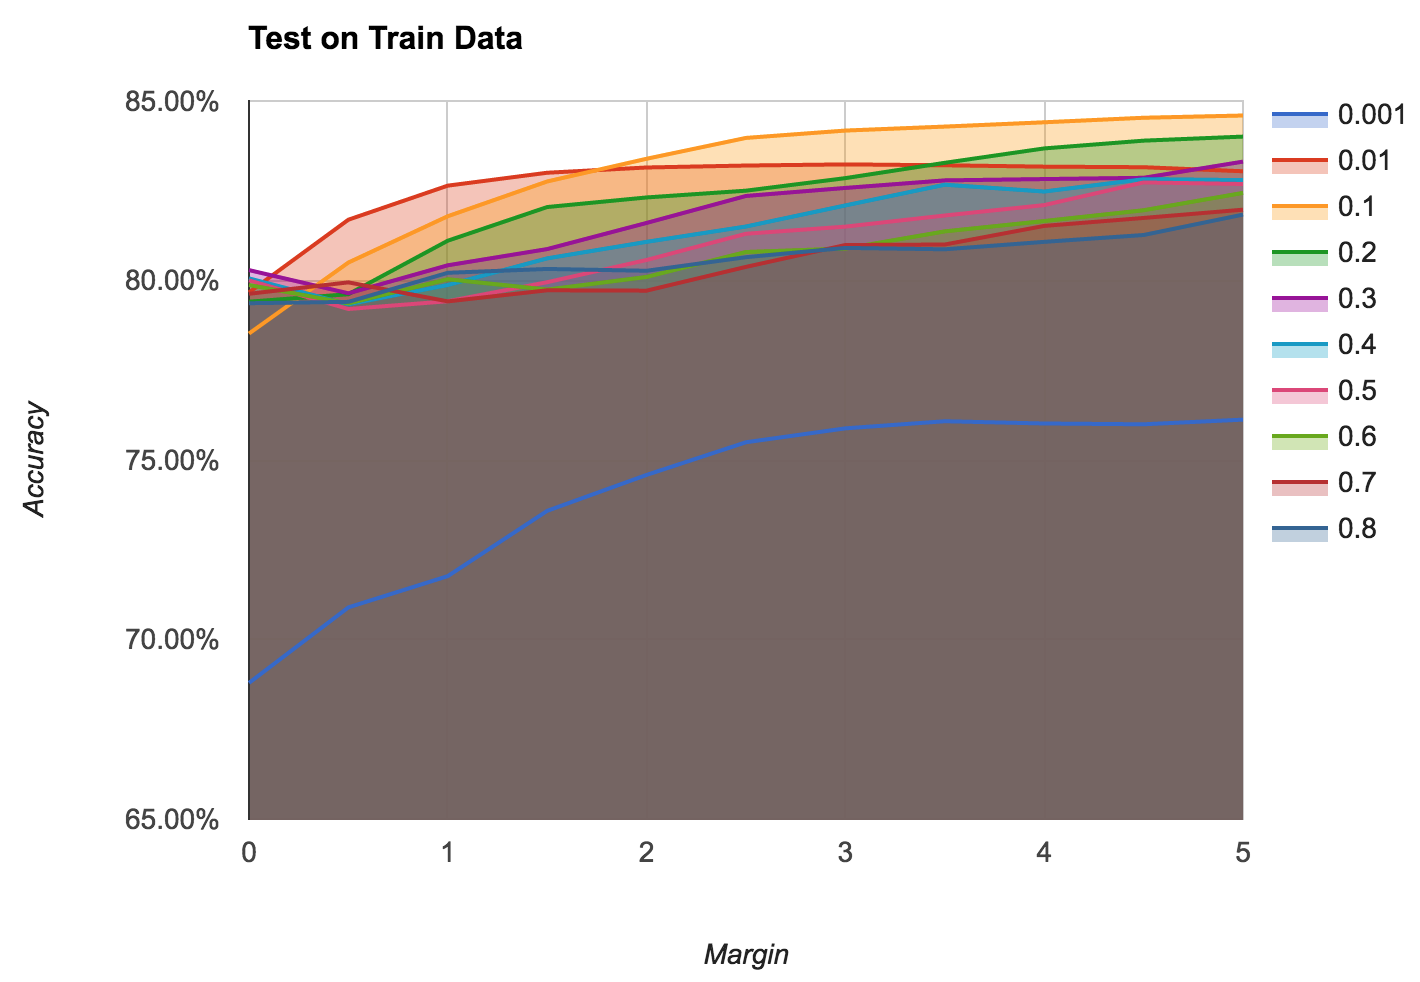
\includegraphics[scale=0.4]{332Train.png}
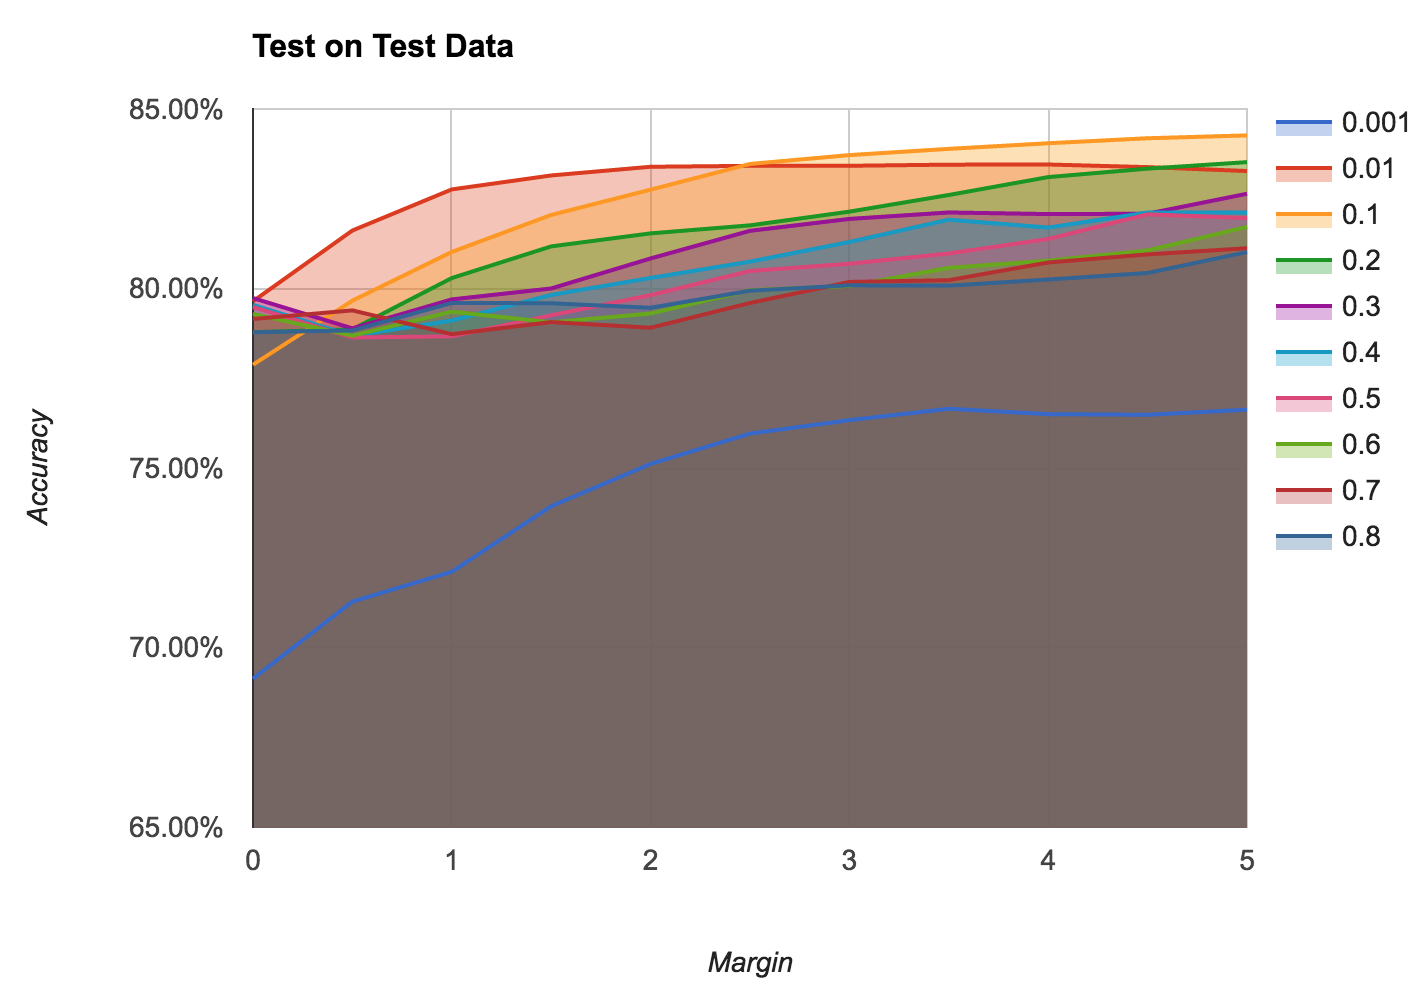
\includegraphics[scale=0.4]{332Test.png}\\
The two graphs represent the margin along the x-axis and accuracy along the y axis. The rate is represented in the legend.\\
We see that the maximum accuracy comes when the rate is 0.1 and the margin is around 5 both while testing on training and test data.\\
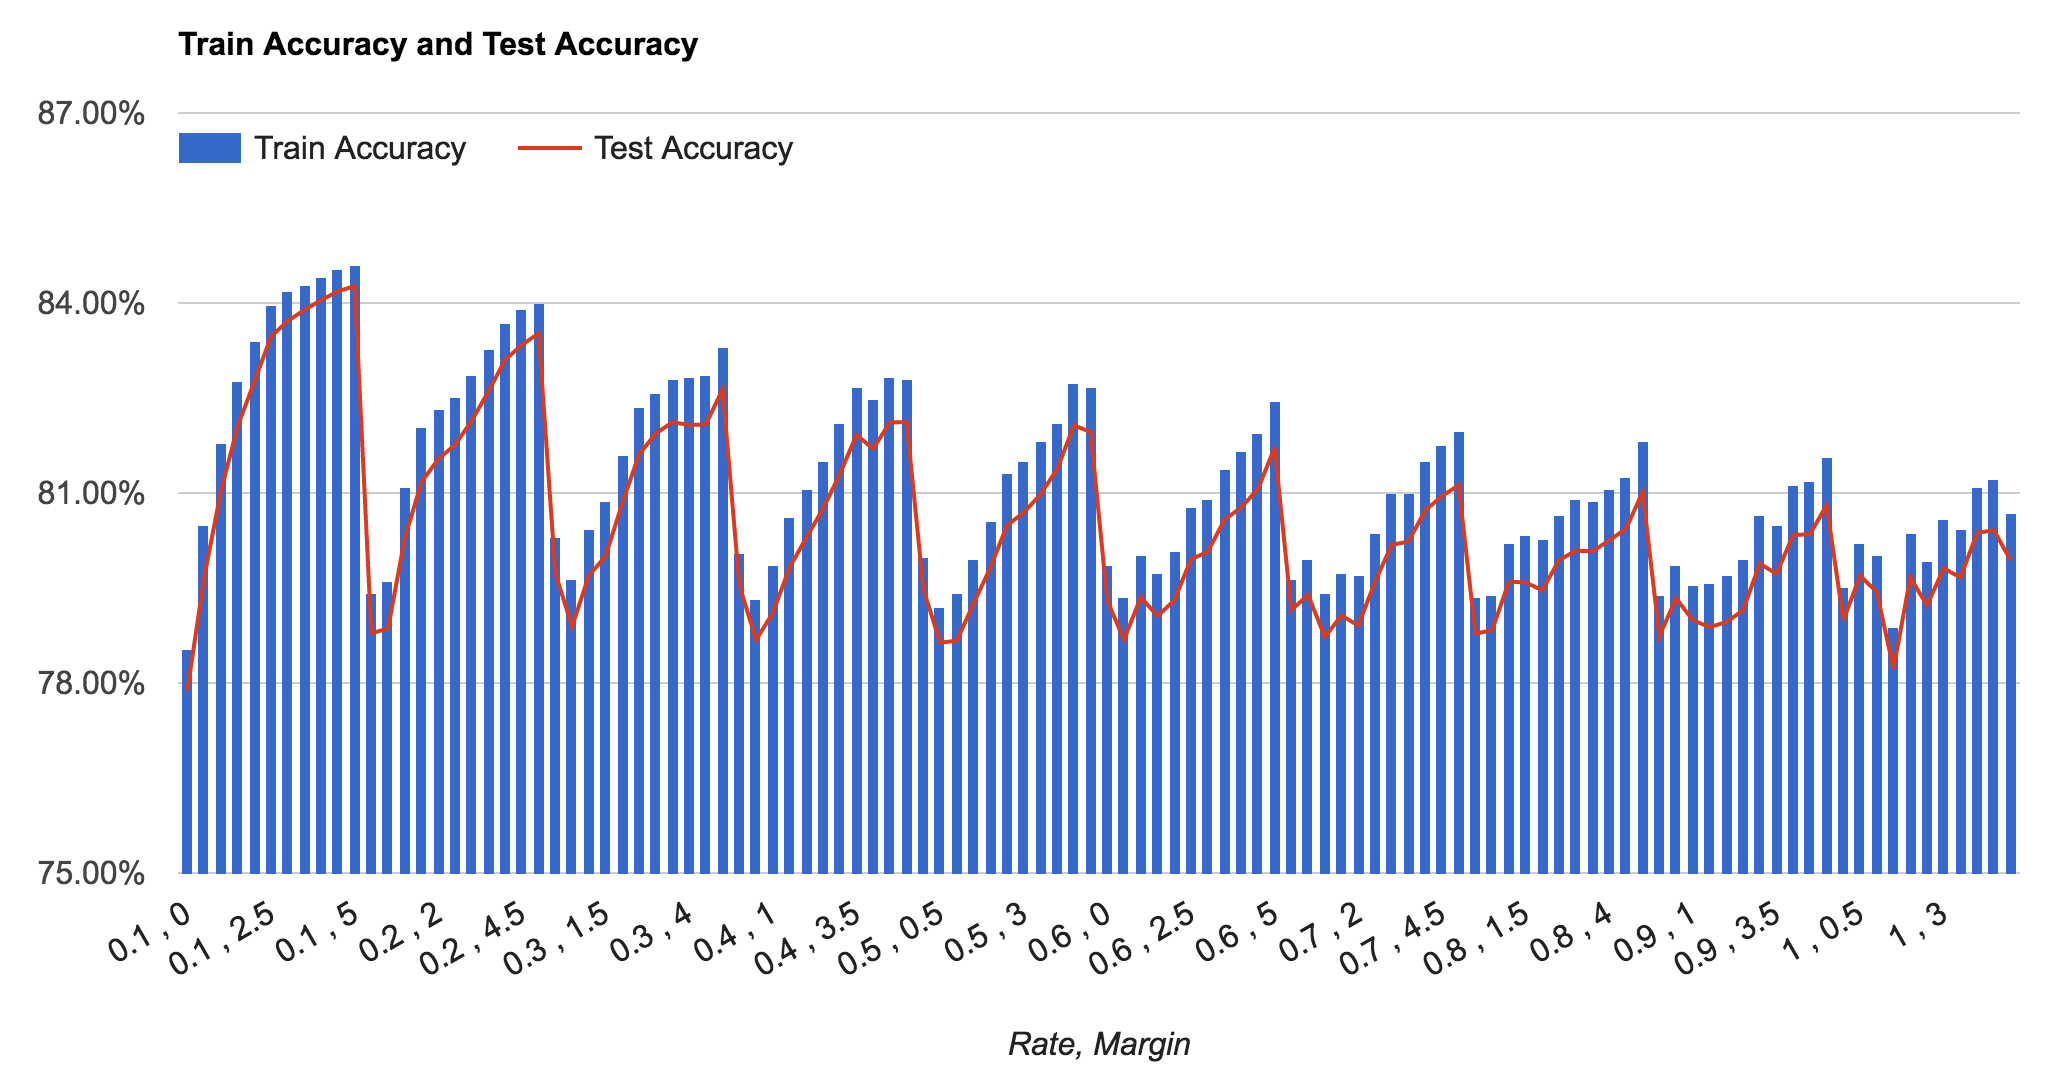
\includegraphics[scale=0.5]{332.png}
For normal perceptron, with rate=0.1:\\ 
Number of updates during training=5784\\
Accuracy on training data during testing=78.5\%\\
Standard Deviation in training data during testing=0.032\\
Accuracy on test data during testing=77.88\%\\
Standard Deviation in test data during testing=0.034\\\\
The maximum accuracy for normal perceptron comes at rate=0.3:\\
Number of updates during training=5299\\
Accuracy on training data during testing=80.29\%\\
Standard Deviation in training data during testing=0.022\\
Accuracy on test data during testing=79.73\%\\
Standard Deviation in test data during testing=0.024\\\\
For margin perceptron performed best  with margin=5 and rate = 0.1,\\
Number of updates during training=5202\\
Accuracy on training data during testing= $84.6\%$ \\
Standard Deviation in training data during testing=0.0016\\
Accuracy on test data during testing=$84.26\%$ \\
Standard Deviation in test data during testing=0.0016\\\\
\emph{A more exhaustive data on this is available in "Outputs/OutputData(3.3.2)"\\
I have reduced the number of iterations in the submitted code as including the exhaustive cases would take a very long time. If required, the values could be changed before execution.}\\\\
3.\\
Here, the program was run under the following setting:\\
1. Number of epochs=3 (no shuffling)\\
2. Number of epochs=3 (with shuffling)\\
3. Number of epochs=5 (no shuffling)\\
4. Number of epochs=5 (with shuffling)\\
Each of the above was run for different  combinations of rate(r) and margin(u). I changed the rate from 0 to 1 in increments of 0.2, and changed margin from 0(normal perceptron) to 5 in increments of 1.\\
Also, since the random initialization of weights were giving different values, I ran each combination of epochs, shuffle, rate and margin for 50 times. Therefore the accuracy and the number of mistakes' values that I have mentioned is the average accuracy and the average number of mistakes over the 50 runs along with its standard deviation for the same rate and margin.\\
The below data summarizes the run. I have attached the raw output for individual runs along with the code in "Outputs/OutputData(3.3.3)" for more details.\\
The below 2 graphs depict the outputs of the multiple runs(one on training data and the other on test).\\
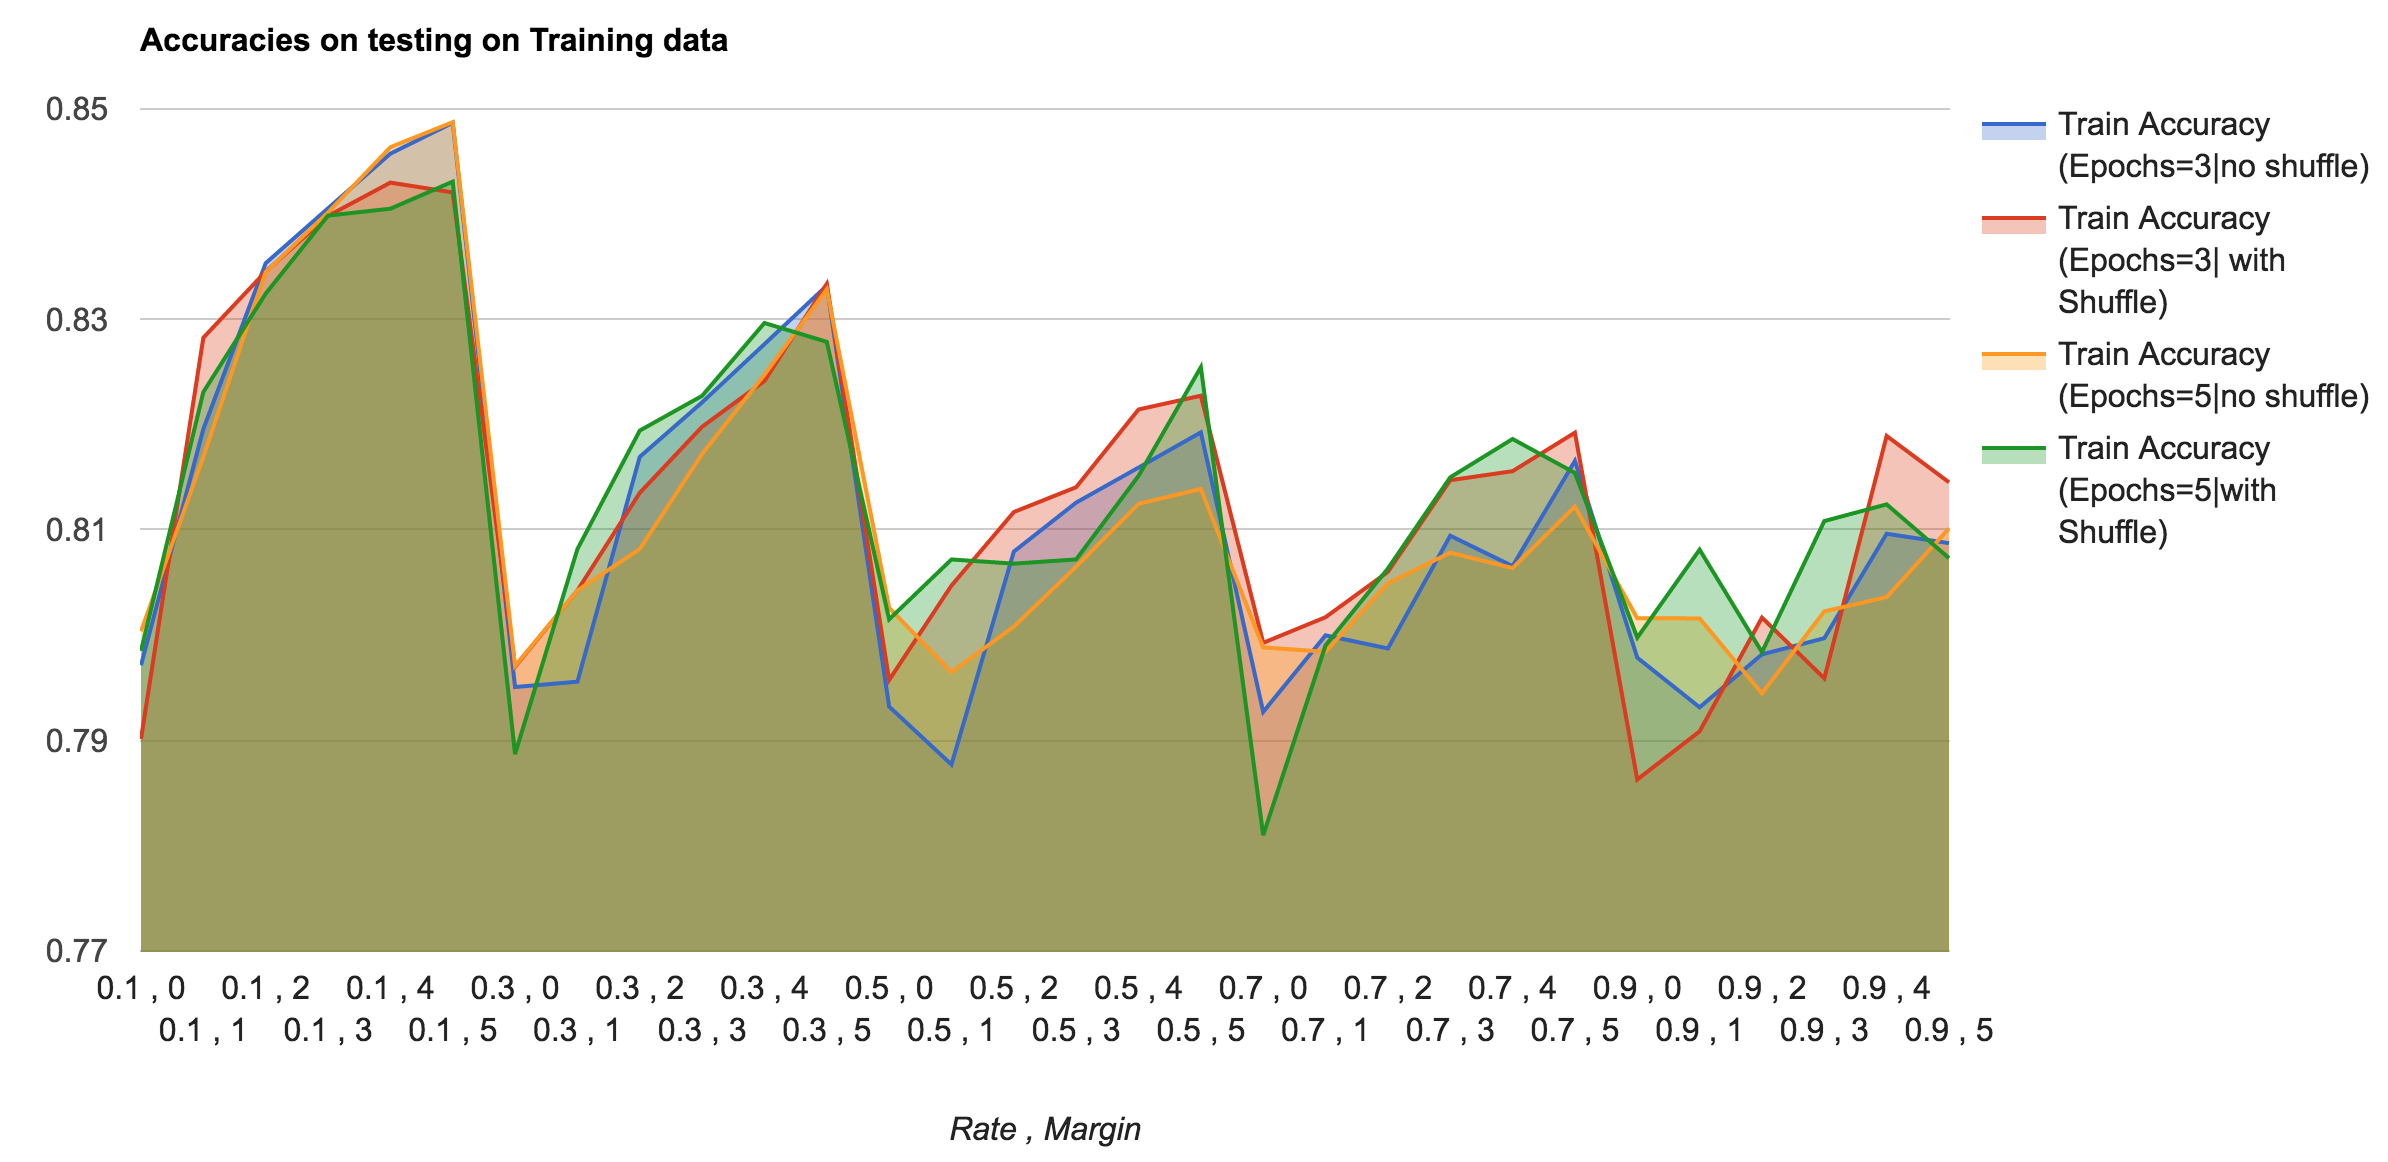
\includegraphics[scale=0.45]{333Train.png}
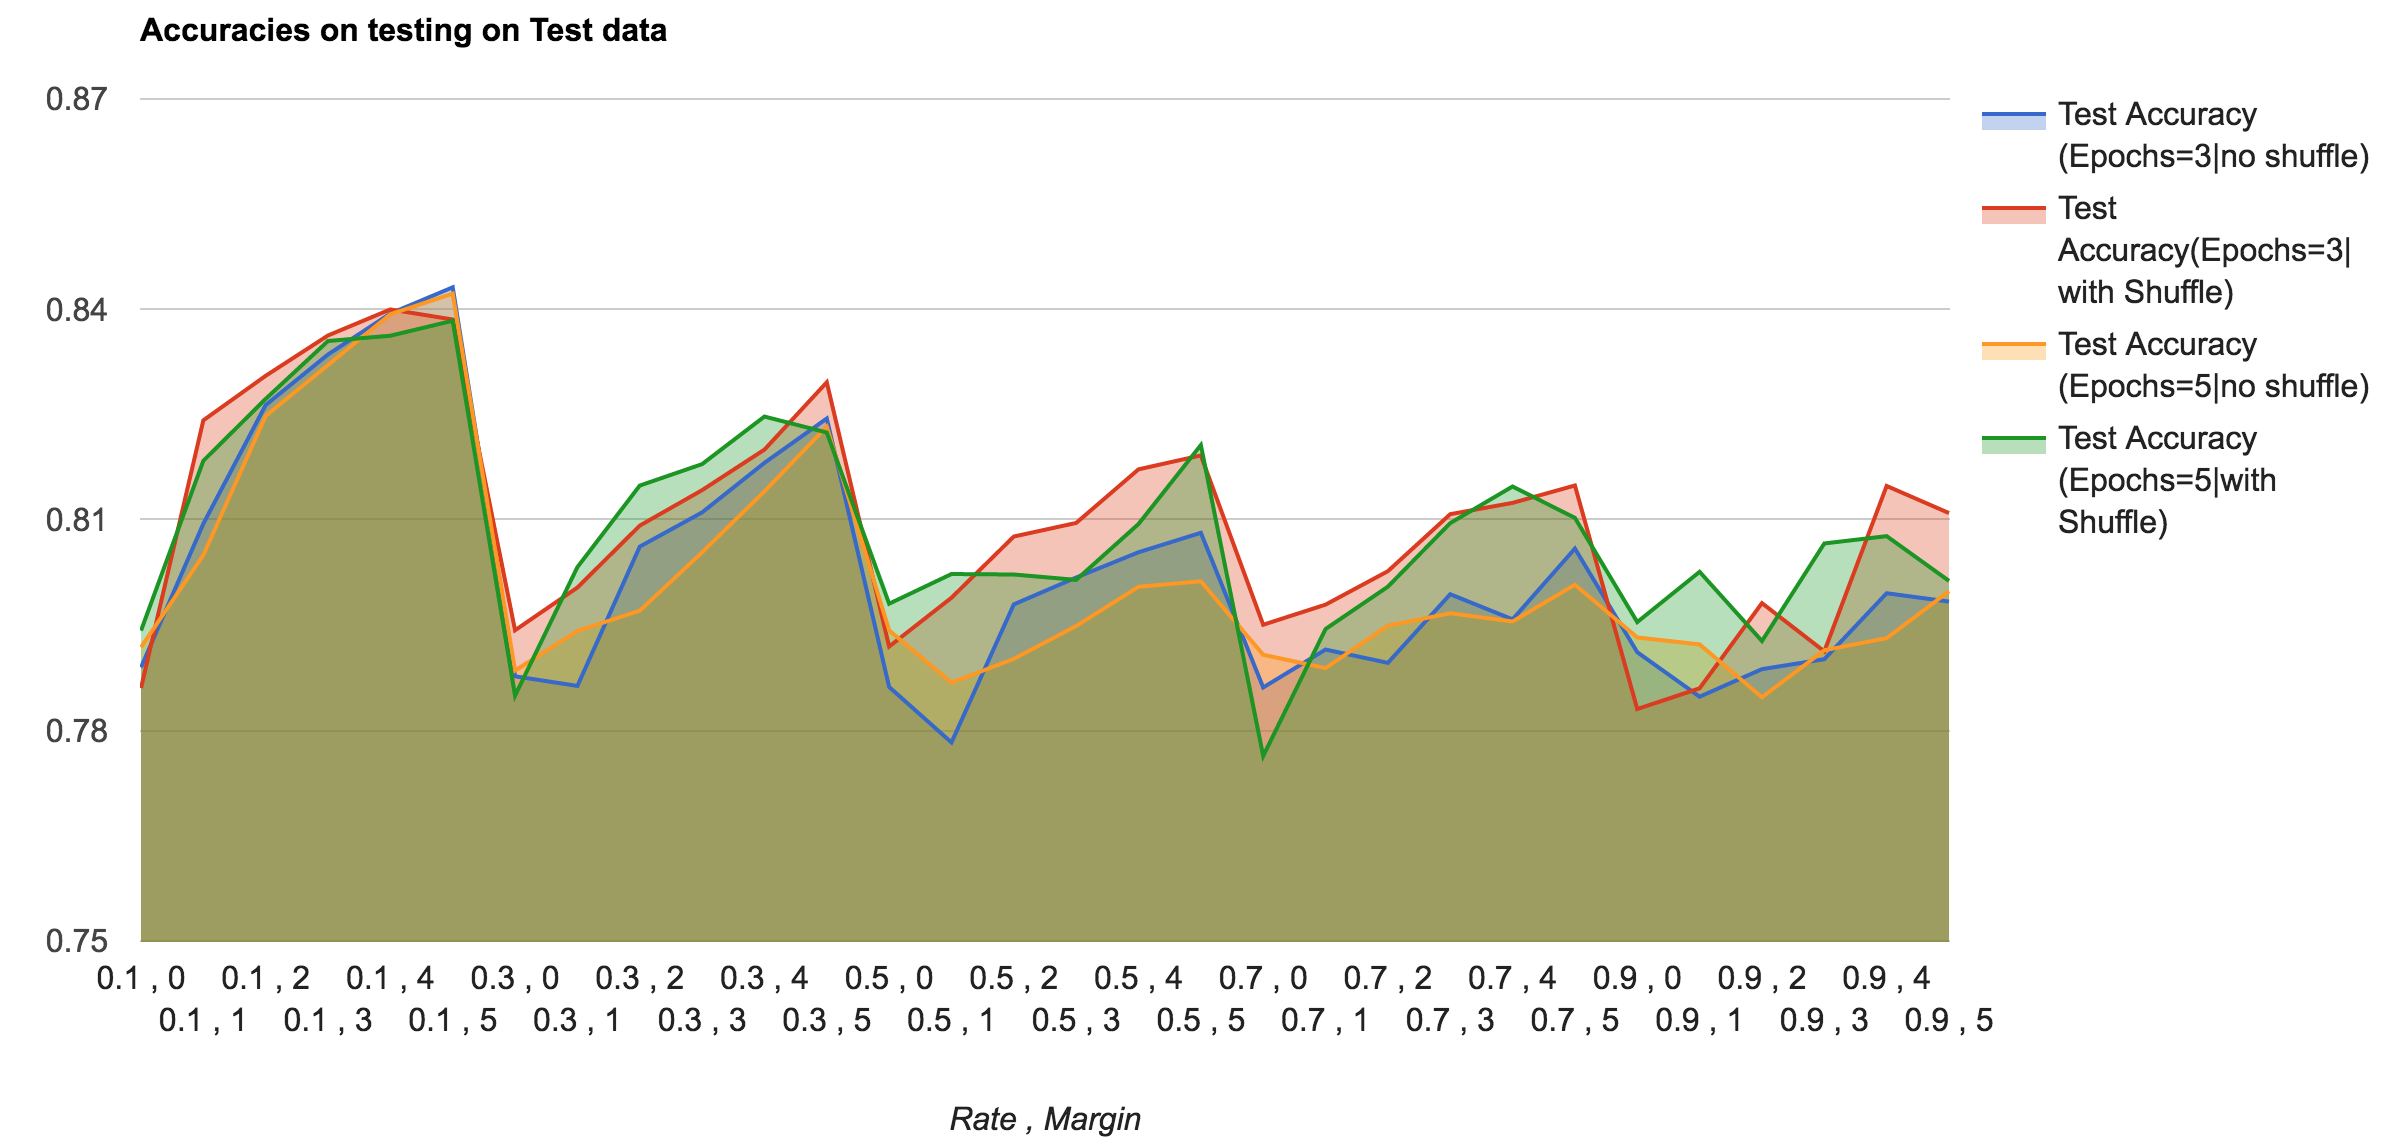
\includegraphics[scale=0.45]{333Test.png}\\
Looking at the graph, overall, it looks like shuffling and increasing the number of epochs is giving a better accuracy. However, the rate and the margin chosen also takes a toll on these values.\\ As seen from the graph, here are the instances with maximum accuracy with different epochs and whether the data is shuffled before every epoch. One table shoes details about the test on training data and the other on test data. Please note the the table shows the instances from the graph above.\\
 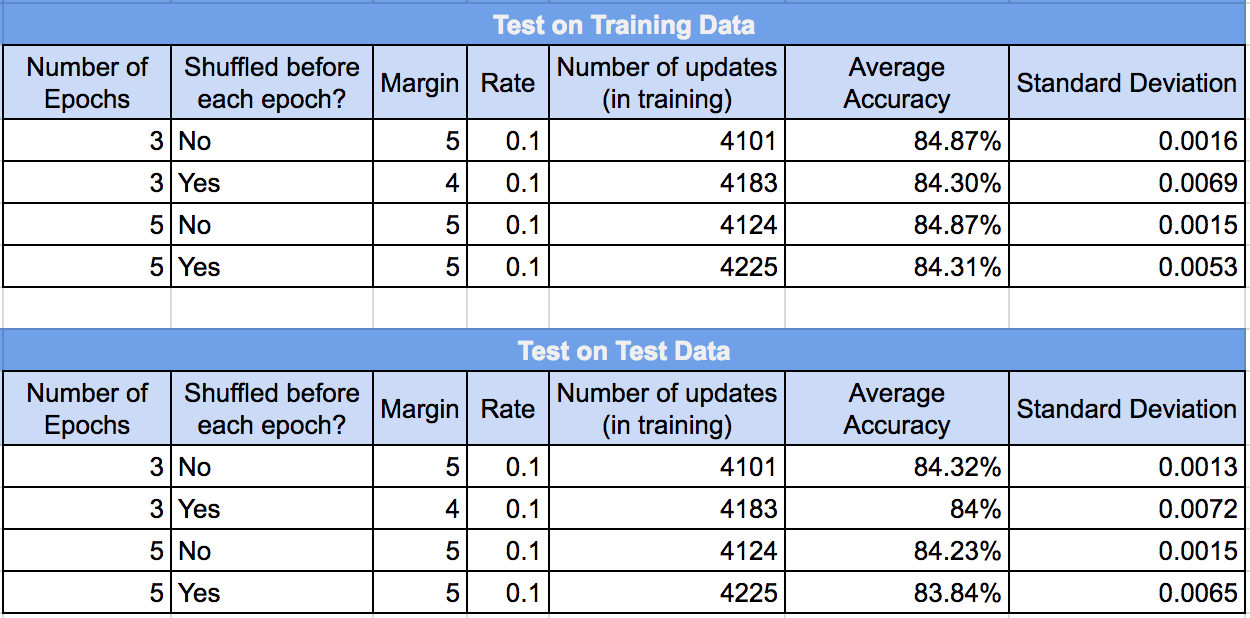
\includegraphics[scale=0.7]{333data.png}\\
 \emph{A more exhaustive data on this is available in "Outputs/OutputData(3.3.2)"\\
I have reduced the number of iterations in the submitted code as including the exhaustive cases would take a very long time. If required, the values could be changed before execution.}\\\\
4.\\
For aggresive perceptron, the program was by training on the train data, and testing on both train and the test data.\\
The program was run for every for normal perceptron and margins from 1 to 5 in increments of 5.\\From the previous data, it is quite clear that for the current data, the perceptron performs best when rate=0.1 and margin=5. However, for aggressive perceptron, I tried to analyze how the margin with effect the different setting of epochs and shuffling. The rate cannot be changed as it is dynamically updated for this setting.\\
Again the program was run for 50 times for each of the setting because of the random assignment of weights. Therefore the accuracy and the number of mistakes' values that I have mentioned is the average accuracy and the average number of mistakes over the 50 runs along with its standard deviation, all other hyper-parameters remaining the same.\\
The below data summarizes the run.I have attached the raw output for individual runs along with the code in "Outputs/OutputData(3.3.4)" for more details.\\
 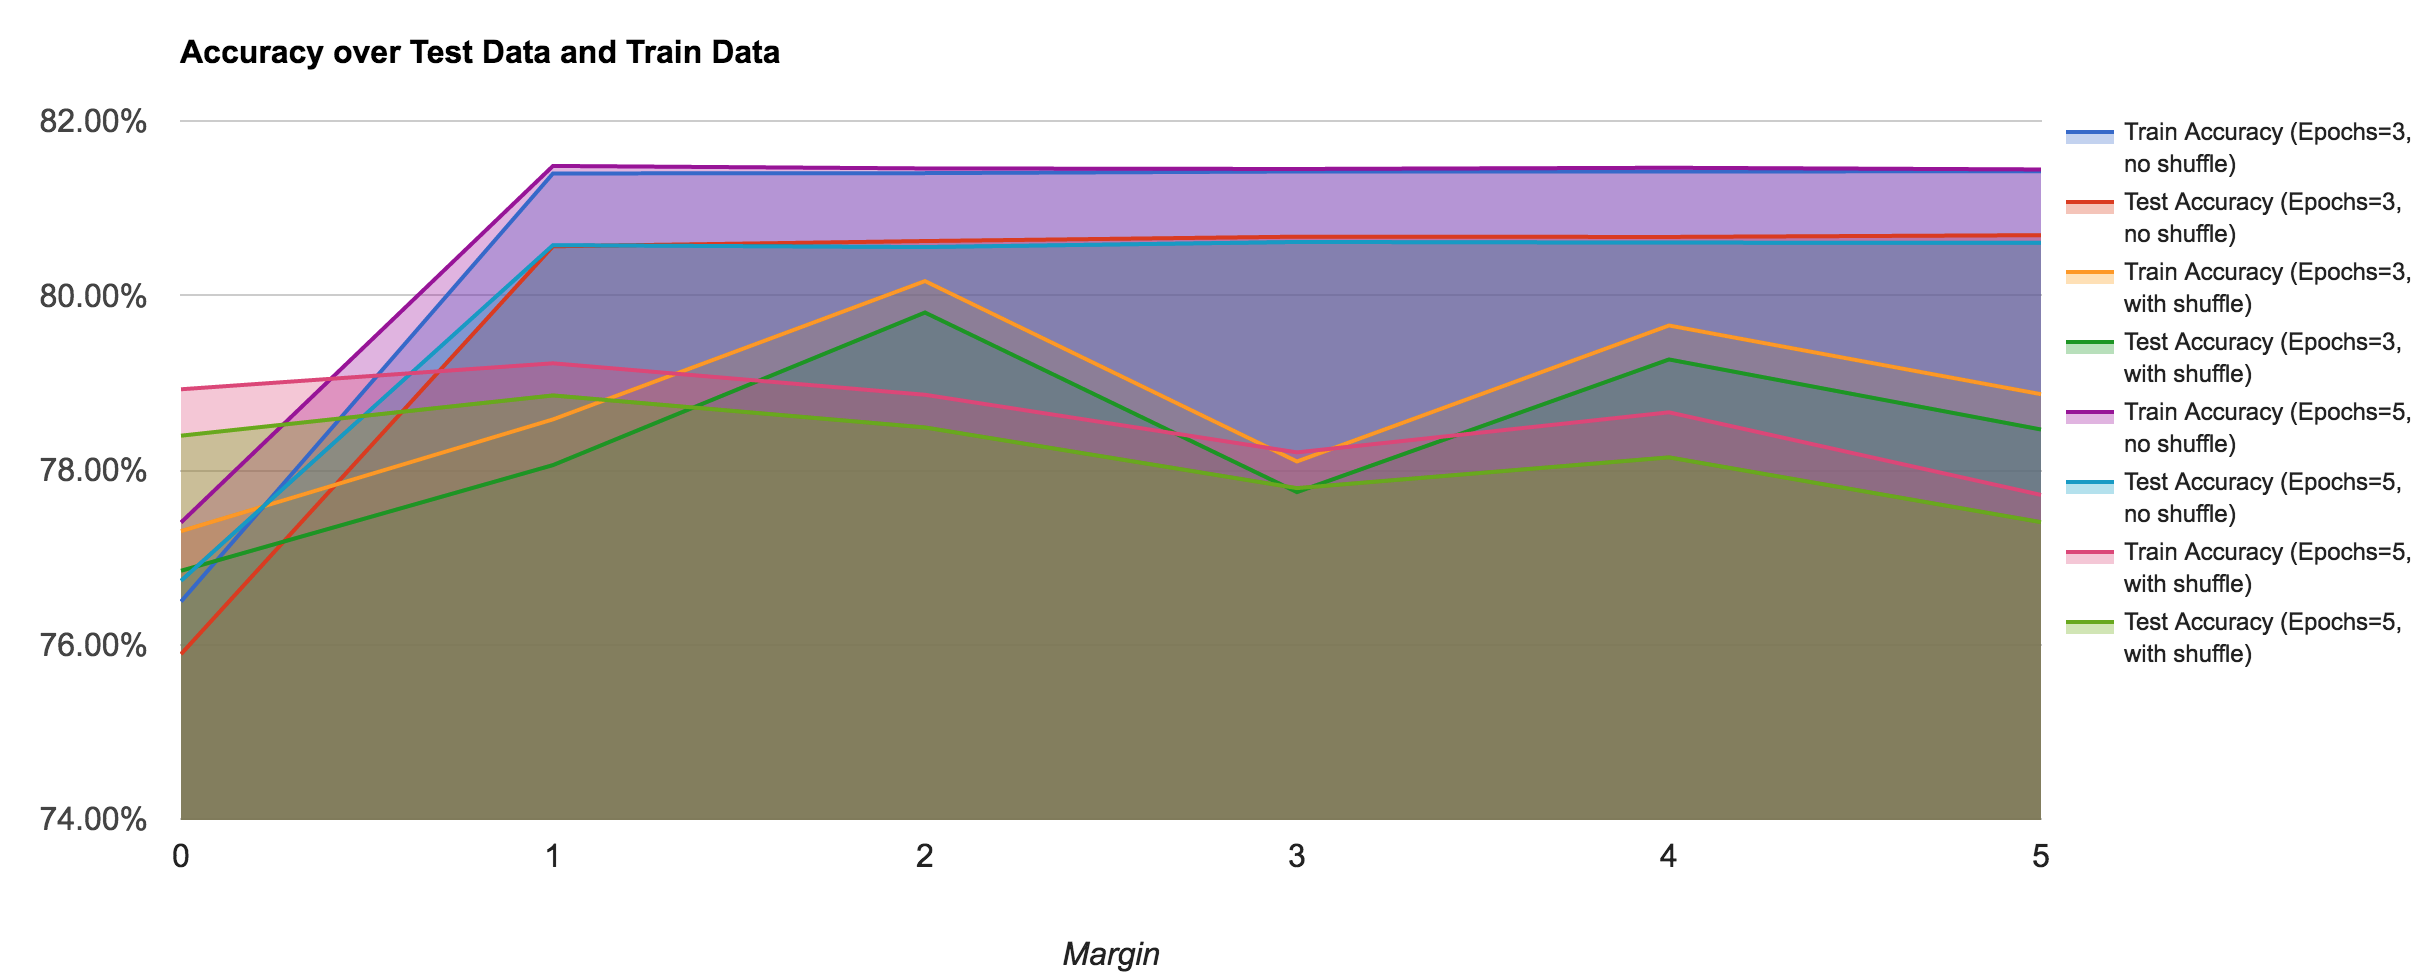
\includegraphics[scale=0.4]{334.png}\\
 \\As we see from the graph, when margin=0(normal perceptron in previous case), does not considerably improve in performance for the aggressive perceptron.\\
 The important thing here is, the accuracy considerably increases with higher margins. This is where the aggressive perceptron actually comes into picture.\\
 With shuffling( with epochs=3 or 5), the accuracy hits upto 84\% at times. The graph and the table below shows a lower value as it is an average over 50 executions, due to random initialization(seeOutputs/OutputData(3.3.4) for the exhaustive data).\\
 An example of the instance from the exhaustive data:  For number of epochs=3, with shuffling, and margin=5,\\
 Number of updates=4543\\
 Accuracy on Training data=83.6\%\\
 Accuracy on Test data=82.62\%\\
 A very important thing to note here is that, without shuffling, as seen in the graph, the accuracy almost remains constant for this data across various margins(>=1). There is a very minute change in the accuracy averaged over 50 runs(even after random weight initializations).\\
 To give a set of values with and without shuffling the data, please find the information below:\\
  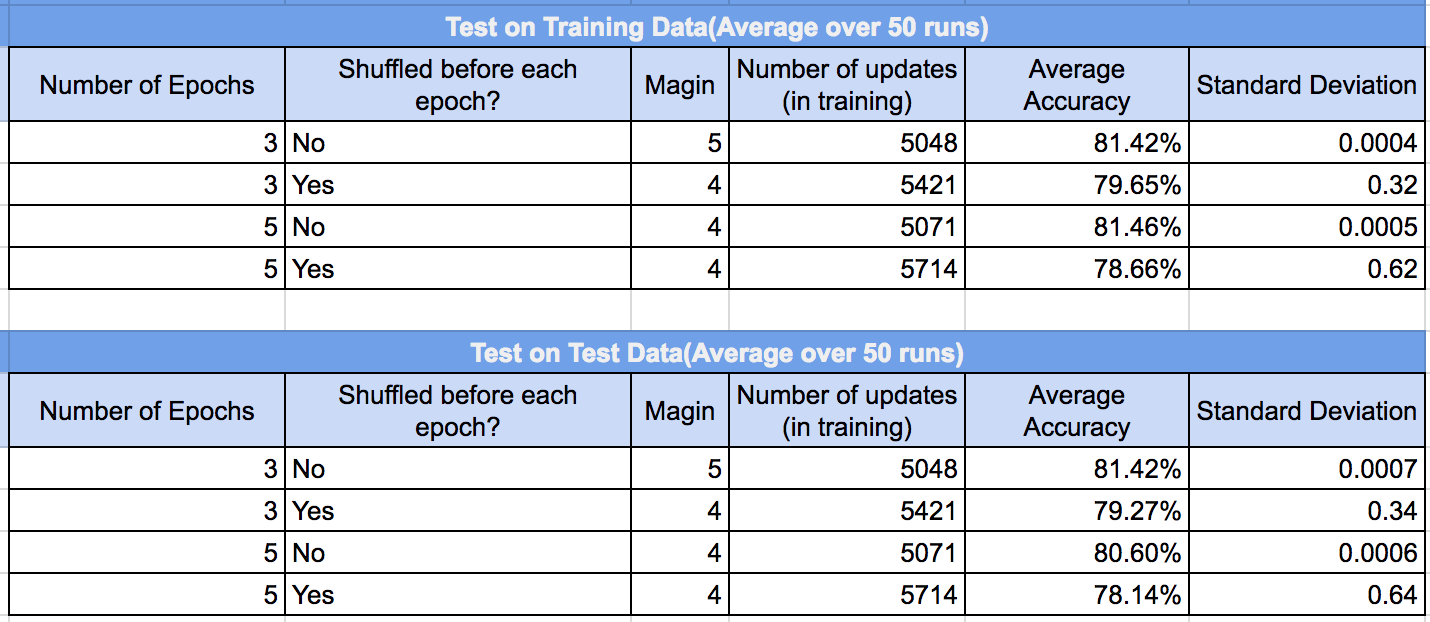
\includegraphics[scale=0.6]{334data.png}\\

 











 



\end{document}
%%% Local Variables:
%%% mode: latex
%%% TeX-master: t
%%% End:
